\chapter{Marco Teórico}
\label{cap:marcoTeorico}

\section{Streaming}

Streaming es una técnica para la transferencia de datos de forma continua, de tal manera que sea temporal y secuencial, cuyo funcionamiento se basa en el envío de datos por parte de un ente externo para que estos sean procesados, y en caso de estar ocupado el servicio, dejar los datos en cola. Generalmente, esto se utilizado en la interacción de usuarios en la Web, como redes sociales, o reproducción \textit{online} de material multimedia. En la Figura \ref{fig:streaming} se muestra un servidor que emana un flujo de datos que llega a distintos clientes, donde cada uno de ellos procesa la información entrante, y en caso de estar ocupado el procesamiento, se guarda en un \textit{buffer} los datos para posteriormente ser procesados.

\begin{figure}[ht!]
  \centering
    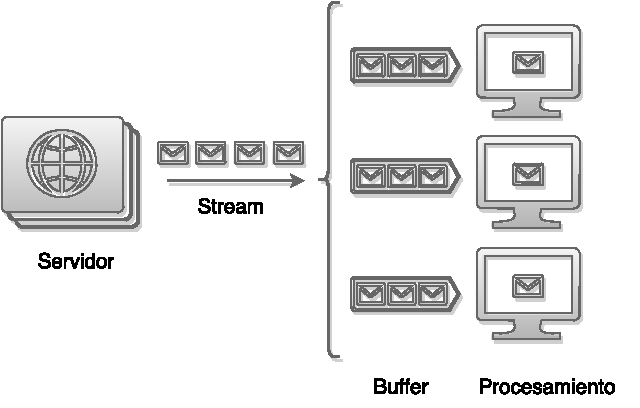
\includegraphics[scale=0.7]{images/Streaming.pdf}
  \caption{Flujo de datos entre servidor y clientes.}
  \label{fig:streaming}
\end{figure}

Este tipo de técnica es útil cuando se desea procesar información en tiempo real, por lo que la temporalidad de los datos es importante, como en la reproducción \textit{online} de datos multimedia. Los datos emanados por el \textit{streaming} pueden ser utiizados para el análisis y procesamiento de una SPS (Sistema de Procesamiento de \textit{Stream}). Un ejemplo de esto es el \textit{Streaming API} proporcionada por Twitter, donde esta información se puede utilizar para estudiar los \textit{trending topic} o los \textit{hashtag} más utilizados para casos en específicos, como campañas políticas o desastres naturales. %Por lo tanto, detección de patrones de la información en el momento, como detección de fraudes, es un buen caso para utilizar como flujo de entrada a los sistemas de procesamiento de \textit{stream}, dado que el flujo de datos está dado por la interacción de transacciones.

En el procesamiento de \textit{stream}, como monitoreo de signos vitales, detección de fraudes, reproducción de videos \textit{online}, es necesario cumplir con ciertos características para el funcionamiento correcto del sistema. Para ello, se han propuesto ciertos requerimientos para el procesamiento continuo de datos \citep{andrade2014fundamentals}, los cuales serán desglosados a continuación:

\begin{itemize}
	\item \textbf{Grandes cantidades de procesamiento de datos distribuidos} Esto significa que algo tratar de procesar los datos, sea tan grande la cantidad de datos a procesaro que no se pueden guardar en una base de datos y realizar \textit{bash processing}. De esta forma, el utilizar \textit{stream processing} soluciona el problema, dado que va procesando mientras van llegando los datos.
	\item \textbf{Estrictas limitaciones de ancho de banda y latencia} Se refiere a la comunicación que existe por parte del proveedor de datos, de tal manera que no sea una limitante en el procesamiento de los datos el ancho de banda o la latencia que existe. Esto es importante, dado que no sirve un sistema de estimación de la bolsa del mercado con datos antiguos, debido a la latencia que existe en el sistema, lo ideal es que se acerquen lo más posible al tiempo real.
	\item \textbf{Procesamiento de datos heterogéneos} En su mayoría, los datos poseen distintos formatos, contenidos y niveles de ruido, por lo que es necesario realizar una normalización de estos, de tal manera de estandarizar el procesamiento.
	\item \textbf{Proporcionar alta disponibilidad a largo plazo} Es importante poseer un constante flujo de información, que sea estable y persistente en el tiempo, de tal manera que constantemente esté procesando los datos para el propósito dado. Por ejemplo, si se posee un sistema de análisis de partículas en el espacio, es necesario que posee una tolerancia a falla, debido que en caso que suceda alguna anomalía pueda seguir funcionando el sistema y procesar la información que se vaya entregando, porque en caso contrario, se perdería el objetivo del procesamiento.
\end{itemize}

\section{Sistemas de Procesamiento de Stream}

Entre los diferentes motores de procesamiento de datos masivos, existen los sistemas de procesamiento de \textsl{stream}, los cuales reciben grandes cantidades de datos que deben procesar de forma distribuida y \textsl{online}. Para realizar esto, se requiere un cambio en el paradigma \textsl{bash processing}, el cual guarda los datos en una base de datos, los que posteriormente son procesados de forma \textsl{offline} \citep{HawwashN14}, a uno que procese de forma \textsl{online}. Por lo que el paradigma cambia a uno basado en grafos, donde los operadores corresponden a las vértices del grafo, y las aristas a los flujos de datos preprocesados que salen del operador, siendo los datos proporcionados por un ente externo, ya sea \textit{streaming} de datos de redes sociales, estadísticas del monitoreo de un sistema u otra información deseada en tiempo real \citep{Shahrivari14}.

El modelo de procesamiento que se muestra en la Figura \ref{fig:grafo}, corresponde a un SPS (Sistema de Procesamiento de \textit{Stream}). Como se había mencionado anteriormente, los vértices corresponden a operadores, como por ejemplo analizadores de sentimientos, filtros de palabras o algún algoritmo en particular, y las aristas corresponden a los flujos de datos entre un operador y otro. Además de esto, se tiene una fuente de datos, la cual entrega los datos iniciales a los primeros operadores del grafo \citep{AppelFFB12}.

\begin{figure}[ht!]
  \centering
    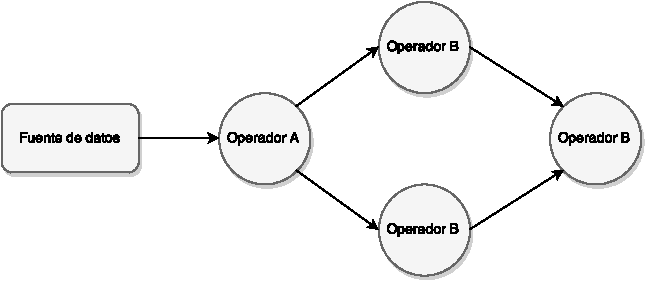
\includegraphics[scale=1]{images/SPS.pdf}
  \caption{Ejemplo de modelo de SPS.}
  \label{fig:grafo}
\end{figure}

Cabe destacar que al ser distribuido los SPS, cada uno de las vértices del grafo serán alojadas en un nodo disponible en el ambiente que se esté almacenado el sistema, ya sea un \textit{cluster}, un \textit{grid} o un \textit{Infrastructure-as-Service}. Por lo que se debe realizar una comunicación entre los distintos nodos, para realizar el envío del flujo de un operador a otro.

Los principales usos que se realizan en los SPS es el manejo de grandes cantidades de información, los cuales son procesados para obtener estadísticas o datos específicos de esto, como es el caso de detección de fraudes, recolección de información en caso de desastres o análisis de la interacción en las redes sociales. Por lo que para efectuar una procesamiento en tiempo real de los datos, se han propuesto los siguientes requerimientos \citep{StonebrakerCZ05}:

\begin{itemize}
	\item \textbf{Baja latencia} Este concepto está asociado con que debe ser fluida la comunicación entre los distintos nodos que estén trabajando en el sistema, de tal manera que no exista \textit{delay} en el procesamiento del sistema.
	\item \textbf{Consultas SQL} Poder realizar consultas a una base de dato, sin perder las propiedades del SPS, como el procesamiento distribuido. Para esto, se debe realizar un cambio en la forma de ejecutar las consultas, debido que no sólo es necesario realizar la consulta, sino también realizar un \textit{merge} de las respuestas, por lo que es necesario otro componente en el sistema.
	\item \textbf{Manejo de fallas en el flujo de dato} Esto significa que es importante poseer sistemas que no se preocupen de la falla en los datos, debido que se posee como premisa que se van a perder datos en el procesamiento de estos, ya sea por las colas, \textit{delay} existente o pérdida de los datos.
	\item \textbf{Generar resultados predecibles} Cuando se realizan consultas en el sistema, puede ser que estas puedan ser correctas en cierto período de tiempo, pero debido a la falla que pueda tener el sistema, el estado de los operadores se pierde y no se obtiene el mismo resultado. Por lo tanto, es importante garantizar que el resultado sea predecible y persistente en el tiempo, de tal manera que si se realiza una consulta, pueda volver a efectuarse un resultado igual u homólogo.
	\item \textbf{Integrar almacenamiento de datos y \textit{Streaming Data}} En general, cuando se trabaja con procesamiento de datos, es importante guardar estados en el sistema, de tal manera que los datos entrantes vayan verificando, modificando o eliminado la información que éste posee. En un contador de palabras, es importante tener variables que vayan guardando las estadísticas del sistema, por lo tanto es indispensable que posea un soporte ante esto. Otro tema importante es la uniformidad de los datos, como se había presentando en el tópico anterior de \textit{Streaming}, siempre se va a trabajar con datos heterogéneos, pero estos deben ser estandarizados para el procesamiento del sistema, de esta manera, no existirá una discordancia en la información procesada.
	\item \textbf{Garantizar la seguridad y disponibilidad de los datos} Este requerimiento está orientado en poseer mecanismos de \textit{checkpoint} y tolerancia a falla, por lo que en caso de existir alguna anomalía, pueda volver el sistema a estar disponible y sin perder una cantidad considerable de información, ya sea en las estadísticas o estados del sistema.
	\item \textbf{Partición y escalabilidad automática de las aplicaciones} Dentro de las consideraciones que se realizan a los SPS es poder distribuir la carta de forma distribuida entre distintos procesadores o máquinas, deseando idealmente una escalabilidad incremental. Si bien no sucede siempre, se espera que esto sea automático y transparente.
	\item \textbf{Procesamiento y respuesta instantánea} Cuando se plantea el uso de los SPS es importante considerar que debe atendar a respuestas lo más cercano al tiempo real, es por esto, que el procesamiento de grandes cantidades de datos debe ser de forma rápida o instantánea. Por lo que es necesario tener una optimización de la sobrecarga que pueda darse, de tal manera que no se haya un alto \textit{overhead} en el sistema.	
\end{itemize}

Cada motor de procesamiento de \textsl{streaming} está basado en un modelo de procesamiento en particular. Por ejemplo, S4 está basado en el modelo de procesamiento \textsl{push} \citep{s4yahoo}, y Storm en el modelo \textsl{pull} \citep{stormtwitter}.

El primer modelo consiste en el envío de datos desde el operador. La ventaja de este modelo empleado por S4 radica en la abstracción en el envío de datos, sin embargo no asegura el procesamiento de estos, debido a que no existe un mensaje de respuesta al ser entregado al operador. En la Figura \ref{fig:sps-push} se puede ver el Operador A como envía los datos al Operador B, donde en caso que esté procesando un dato el Operador B, éste lo guardará en cola. No existe algún mecanismo para asegurar que llegue efectivamente el dato, puede darse el caso que por falla de la red no se haya enviado u otro motivo, por lo que existe una abstracción en el envío de los datos.

\begin{figure}[ht!]
  \centering
    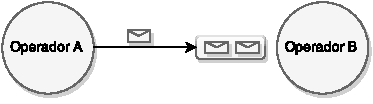
\includegraphics[scale=1]{images/SPS-Push.pdf}
  \caption{Modelo push.}
  \label{fig:sps-push}
\end{figure}

En cambio, en el segundo modelo se basa en la petición de datos a un operador, por lo que son enviados solo si son requeridos. Si bien este modelo asegura procesamiento de los datos, genera una menor abstracción al programador, dado que en el primer modelo sólo se indica a que operador deben ir los datos, en cambio en el segundo se debe indicar quién lo envía y quién lo recibe. En la Figura \ref{fig:sps-pull} se puede ver que existen dos operadores, donde en la parte (a) se solicita por parte del Operador B el envío de un dato para ser procesado, donde en la parte (b) el Operador A envía el dato para que posteriormente sea procesado por el Operador B.

\begin{figure}[ht!]
  \centering
    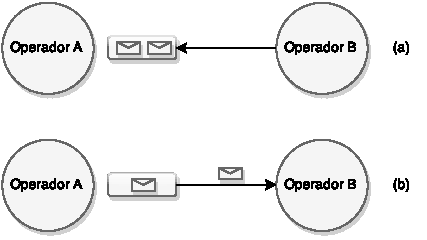
\includegraphics[scale=1]{images/SPS-Pull.pdf}
  \caption{Modelo pull.}
  \label{fig:sps-pull}
\end{figure}

\section{Procesos estocásticos}
Se define proceso estocástico como una colección de variables aleatorias {$X_t$, con $t \epsilon T$}, las cuales están determinadas por algún comportamiento en el tiempo $t$. Esto significa que cada variable estará tratada de forma discreta en el tiempo, sin poseer un proceso determinístico entre sus variables, es decir, que las variables dependan de la historia \citep{taylor2014introduction}.

Por lo tanto, se puede definir estado como el posible comportamiento que puede tener una variable aleatoria en el sistema. Por ejemplo, se puede poseer un modelo que considere tres estados: estable, inestable y ocioso, y según el valor de la variable aleatoria pueda definirse el estado en uno de esos tres estados. Dado estos estados, puede generarse modelos que aplican estos estados como las cadenas de Markov, las cuales toman representan distintos estados dada variables aleatorias en tiempos discretos y una serie temporal con sus respectivas variables aleatorias \citep{de1978calculus}.

\subsection{Cadena de Markov}
Sea $X_t$ el valor de una variable aleatoria $X$ en un tiempo $t$. El conjunto de todas los valores posibles para $X$ se llama espacio de estado \citep{ching2006markov}. La variable aleatoria es un proceso de Markov si las probabilidades de transición entre dos estados cualquiera de $\omega$ sólo depende del estado, lo cual se denota en la Ecuación \ref{eq:defMarkov} y gráficamente en la Figura \ref{fig:procesoMarkov}. Cabe destacar que este tipo de proceso es un caso específico de los procesos estocásticos.

\begin{equation} \label{eq:defMarkov} 
	P_r(X_{t+r} = S_j | X_0 = S_k ; X_1 = S_l ; ... ; X_t = S_i) = P_r(X_{t+1} = S_j | X_t = S_i)
\end{equation}

\begin{figure}[ht!]
  \centering
    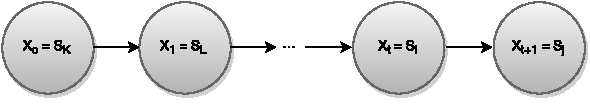
\includegraphics[scale=0.6]{images/ProcesoMarkov.pdf}
  \caption{Proceso de Markov.}
  \label{fig:procesoMarkov}
\end{figure}

Una cadena de Markov es una secuencia de variables aleatorias generadas por un proceso de Markov, como se denota en la Ecuación \ref{eq:cadenaMarkov}

\begin{equation} \label{eq:cadenaMarkov}
	(X_0, X_1, X_2, ..., X_{n-1}, X_{n})
\end{equation}

La cual se define por sus probabilidades de transición, definida en la Ecuación \ref{eq:cadenaMarkov}. En la Figura \ref{fig:cadenaMarkov} se muestra un ejemplo de la transición del estado $i$ al estado $j$, dada la probabilidad $P_{ij}$.

\begin{equation} \label{eq:transicionMarkov}
	P_{ij} = P_r(i \rightarrow j) = P_r(X_{t+1} = S_j | X_t = S_i)
\end{equation}

\begin{figure}[ht!]
  \centering
    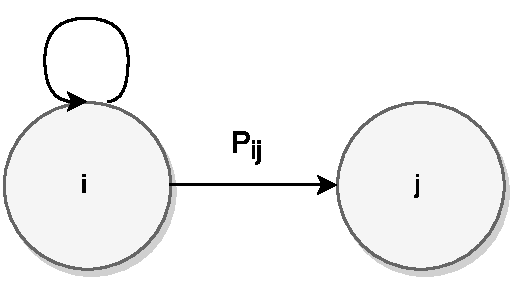
\includegraphics[scale=0.6]{images/CadenaMarkov.pdf}
  \caption{Cadena de Markov.}
  \label{fig:cadenaMarkov}
\end{figure}

En la Ecuación \ref{eq:matrizTransicion} se presenta una matriz de transición de finitos estados, donde la probabilidad de pasar de un estado a otro esta terminado por una posición de la matriz, tomando en consideración que la suma de todas las transición de un estado debe ser igual a 1.

\begin{equation} \label{eq:matrizTransicion}
	P =
	\begin{bmatrix}
		P_{1,1} & P_{1,2} & \cdots & P_{1,n} \\
		P_{2,1} & P_{2,2} & \cdots & P_{2,n} \\
		\vdots  & \vdots  & \ddots & \vdots  \\
		P_{n,1} & P_{n,2} & \cdots & P_{n,n} \\
	\end{bmatrix}
	\hspace*{1cm} \sum_{j=1}^{n} P_{ij} = 1 ; \forall i
\end{equation}

En la Figura \ref{fig:ejCadenaMarkov} se muestra un ejemplo de una cadena de Markov simple, donde se analiza la probabilidad del clima de mañana dado el clima de hoy día. Como se podrá observar, no se considera la historia del clima en la semana, sólo en el caso actual, lo cual es aplicado en los procesos estocásticos. Dada las probabilidades que transite de un clima a otro, se puede ver en la Ecuación \ref{eq:ejCadenaMarkov} la matriz de transición resultante.

\begin{figure}
	\centering
	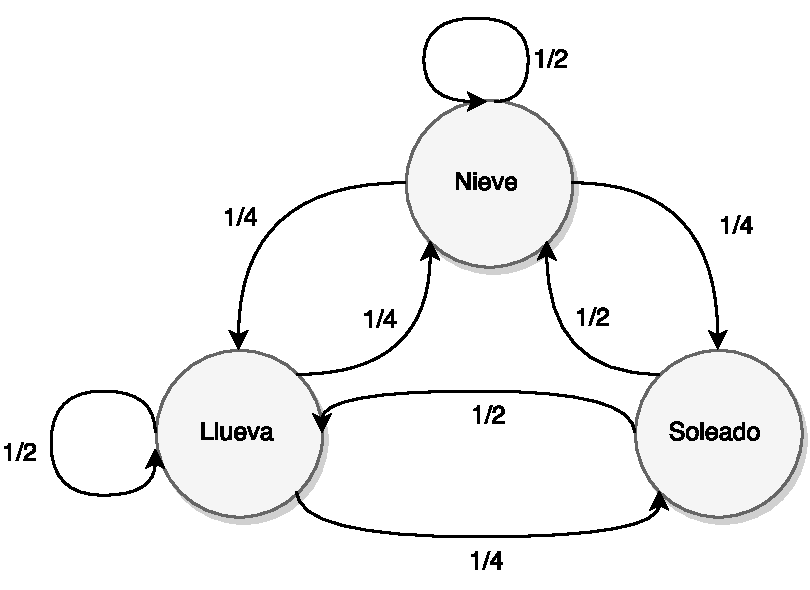
\includegraphics[scale=0.5]{images/EjCadenaMarkov.pdf}
	\caption{Ejemplo de cadena de Markov.}
	\label{fig:ejCadenaMarkov}
\end{figure}

\begin{equation} \label{eq:ejCadenaMarkov}
	P =
	\begin{bmatrix}
		\frac{1}{2} & \frac{1}{4} & \frac{1}{4} \\
		\frac{1}{2} & 0 & \frac{1}{2} \\
		\frac{1}{4} & \frac{1}{4} & \frac{1}{2}
	\end{bmatrix}	
\end{equation}

Si se desea saber la probabilidad que la cadena esté en el estado $S_i$ en el tiempo $t+1$, está dada por la ecuación de Chapman-Kolmogórov \citep{Papoulis1984}:

\begin{equation} \label{eq:chapman-kolmogorov1}
\begin{split}
	\Pi_{i} (t+1) &= P_r(X_{t+i}=S_i) \\
				  &= \sum _{k} P_r(X_{t+i} = S_i / X_t = S_k)·P_r(X_t = S_k)\\
				  &= \sum _{k} P_r(X_{t+i} = S_i / X_t = S_k)·\Pi_{k} (t)
\end{split}	
\end{equation}

En notación matricial:

\begin{equation} \label{eq:chapman-kolgorov2}
\begin{split}
	\Pi_{(t+1)} &= \Pi_{(t)}P\\
	\begin{bmatrix}
		\Pi_1 & \Pi_2 & \Pi_3
	\end{bmatrix} _{(t+1)}
	&= \begin{bmatrix}
		\Pi_1 & \Pi_2 & \Pi_3
	\end{bmatrix} _{(t)}
	\begin{bmatrix}
		P_{1,1} & P_{1,2} & \cdots & P_{1,n} \\
		P_{2,1} & P_{2,2} & \cdots & P_{2,n} \\
		\vdots  & \vdots  & \ddots & \vdots  \\
		P_{n,1} & P_{n,2} & \cdots & P_{n,n}
	\end{bmatrix}
\end{split}
\end{equation}

Usando recurrencia, se puede calcular la distribución estacionaria como se muestra la ecuación \ref{eq:chapman-kolgorov3}, la cual indica el comportamiento a futuro de la cadena de Markov, dado los estados y transiciones que éste posee.

\begin{equation} \label{eq:chapman-kolgorov3}
\begin{split}
	\Pi (t) &= \Pi (t-1)P \\
				  &= \Pi (t-2)P^{2}\\
				  &= \Pi (0)P^{t} ; \Pi (0): \text{distribución inicial}
\end{split}
\end{equation}

\subsection{Trabajo relacionado}
Los modelos predictivos están basados en modelos matemáticos, los cuales simulan el comportamiento del sistema, ya sea del flujo o de la carga de un operador, de tal manera que pueda predecir como será su estado en un tiempo futuro. En general, para poder realizar una predicción se analiza las variables deseadas en una ventana de tiempo, para posteriormente aplicar un modelo matemático que prediga la variación del sistema en la próxima ventana de tiempo que se tiene estipulada.

Dentro de las aplicaciones que se han realizado con modelos predictivos, se encuentra PRESS \citep{GongGW10}. En este sistema orientado para \textit{Cloud Computing}, lo que se analiza es la cantidad de recursos disponibles, ya sea la memoria disponible o el uso promedio de CPU, en las máquinas virtuales que se dispone en el \textit{Infrastructure-as-a-Service}. Para realizar la predicción del estado del sistema, se aplicó cadenas de Markov, tomando sus estados como ventanas de tiempo en un determinado período. De esta manera, se analiza el estado del sistema en un tiempo en específico, para analizar si posee correlación con algún estado de la cadena de Markov, para posteriormente ver la transición de ese estado a otro y generar la matriz de transición. Posteriormente, con la ecuación de Chapman-Kolmogorov, se calcula la distribución estacionaria de la matriz estacionaria, de tal manera de saber en que estado estará en la próxima ventana de tiempo, para finalmente analizar si es necesario algún cambio en el sistema.

Dentro de la misma línea de modelos predictivos, existe el sistema AGILE \citep{NguyenSGSW13} para \textit{Cloud Computing}, que modifica las máquinas virtuales de forma elástica en un \textit{Infrastructure-as-a-Service}. Lo que se realizó en este trabajo fue aplicar la transformada de Fourier \citep{falk2012first} a la carga de CPU en una ventana de tiempo determinada, donde la función resultante se analizó con distintas frecuencias, de tal manera de solicitar la predicción de la próxima ventana de tiempo a cada una de las funciones creadas. De esta manera, se sintetizan todas predicciones realizadas por cada función, para analizar el comportamiento del sistema en la próxima ventana de tiempo, y ver si es necesario aumentar o disminuir recursos de éste.

\section{Teoría de colas}

%Pues bien, independiente del método que se utilice, existe un problema en la distribución, dado el dinamismo de los datos a procesar, pudiendo generarse sobrecargas en algún operador. Esto se produce dado que la tasa de procesamiento es menor a la tasa de llegada, generando colas en el sistema \citep{queueingtheory}. Por ejemplo, si se posee una tasa de llegada $\lambda$ y una tasa de servicio $\mu$, donde $\mu < \lambda$, se generan colas en el sistema, debido que se procesa más lento de lo que llegan los datos. Como existen colas, es necesario un aumento del rendimiento del sistema, debido que $\rho > 1 $, donde se define $\rho = \frac{\lambda}{s\mu}$, siendo $s$ la cantidad de servicios disponibles.

Dentro de los sistemas que se basan en el modelo de productor y consumidor, puede tratarse como un modelo matemática basado en las líneas de espera en el sistema, el estudio de esto se denomina teoría de colas.

La teoría de colas se centra en el estudio de las colas que existen en un sistema cuyo esquema existe un productor y un consumidor (servidor), como se muestra en la Figura \ref{fig:teoriaColas}. En este esquema se puede ver que existe 

\begin{figure}
	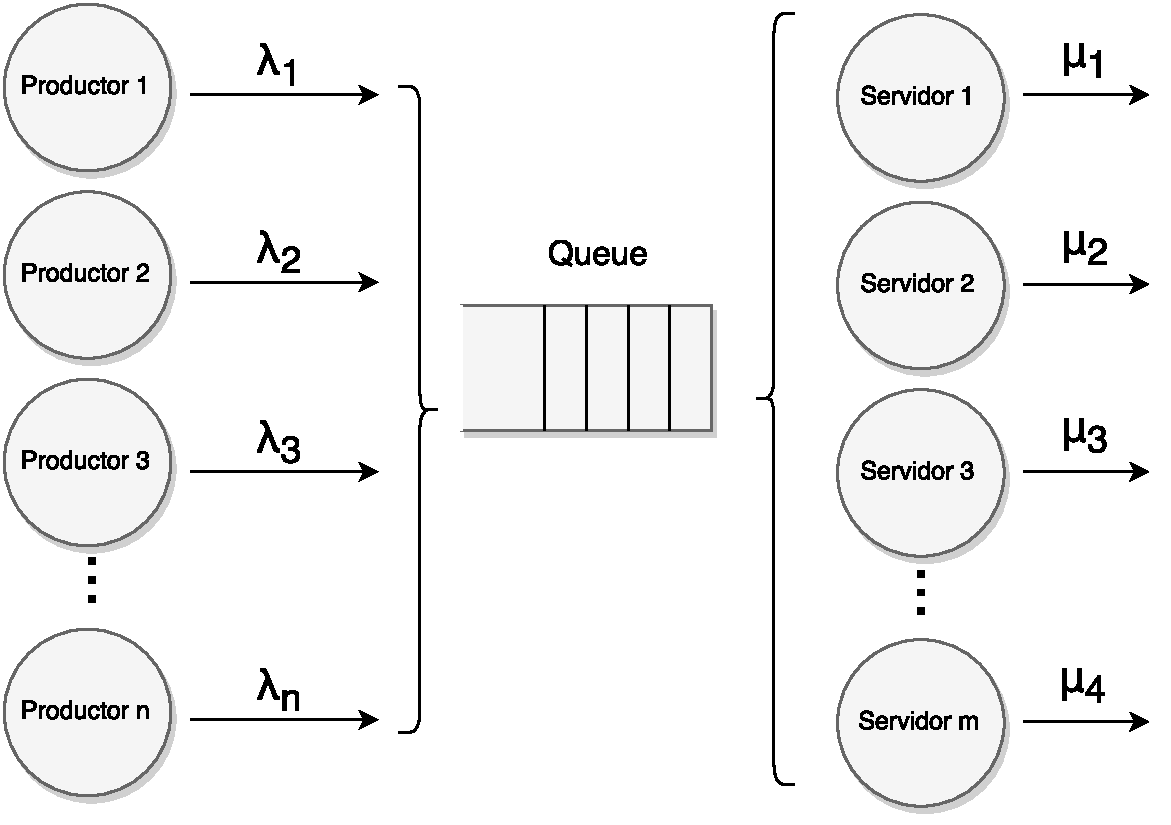
\includegraphics[scale=1]{images/TeoriaColas.pdf}
	\caption{Ejemplo de un sistema.}
	\label{fig:teoriaColas}
\end{figure}